\documentclass{beamer}
\usepackage{fontspec}
\usepackage{bibentry}
\setmainfont{Times-Roman}
\setsansfont{SourceSerifPro-Regular}
\setmonofont{CascadiaCode}
\setbeamertemplate{frametitle}[default][center]

\mode<presentation> {

% The Beamer class comes with a number of default slide themes
% which change the colors and layouts of slides. Below this is a list
% of all the themes, uncomment each in turn to see what they look like.

\usetheme{default}
%\usetheme{AnnArbor}
%\usetheme{Antibes}
%\usetheme{Bergen}
%\usetheme{Berkeley}
%\usetheme{Berlin}
%\usetheme{Boadilla}
%\usetheme{CambridgeUS}
%\usetheme{Copenhagen}
%\usetheme{Darmstadt}
%\usetheme{Dresden}
%\usetheme{Frankfurt}
%\usetheme{Goettingen}
%\usetheme{Hannover}
%\usetheme{Ilmenau}
%\usetheme{JuanLesPins}
%\usetheme{Luebeck}
%\usetheme{Madrid}
%\usetheme{Malmoe}
%\usetheme{Marburg}
%\usetheme{Montpellier}
%\usetheme{PaloAlto}
%\usetheme{Pittsburgh}
%\usetheme{Rochester}
%\usetheme{Singapore}
%\usetheme{Szeged}
%\usetheme{Warsaw}

% As well as themes, the Beamer class has a number of color themes
% for any slide theme. Uncomment each of these in turn to see how it
% changes the colors of your current slide theme.

%\usecolortheme{albatross}
%\usecolortheme{beaver}
%\usecolortheme{beetle}
%\usecolortheme{crane}
%\usecolortheme{dolphin}
\usecolortheme{dove}
%\usecolortheme{fly}
%\usecolortheme{lily}
%\usecolortheme{orchid}
 %\usecolortheme{rose}
%\usecolortheme{seagull}
%\usecolortheme{seahorse}
%\usecolortheme{whale}
%\usecolortheme{wolverine}

%\setbeamertemplate{footline} % To remove the footer line in all slides uncomment this line
%\setbeamertemplate{footline}[page number] % To replace the footer line in all slides with a simple slide count uncomment this line

%\setbeamertemplate{navigation symbols}{} % To remove the navigation symbols from the bottom of all slides uncomment this line
}

\usepackage{graphicx} % Allows including images
\usepackage{booktabs} % Allows the use of \toprule, \midrule and \bottomrule in tables

%----------------------------------------------------------------------------------------
%	TITLE PAGE
%----------------------------------------------------------------------------------------

\title[Short title]{General Video Game playing AI: A Survey} % The short title appears at the bottom of every slide, the full title is only on the title page

\author{ Wangzhihui Mei 2019124044} % Your name
\institute[JI] % Your institution as it will appear on the bottom of every slide, may be shorthand to save space
{
CCNU-UOW JI \\ % Your institution for the title page
\medskip
\textit{maywzh@gmail.com} % Your email address
}
\date{\today} % Date, can be changed to a custom date

\begin{document}

\begin{frame}
\titlepage % Print the title page as the first slide
\end{frame}

\begin{frame}
\frametitle{Overview} % Table of contents slide, comment this block out to remove it
\tableofcontents % Throughout your presentation, if you choose to use \section{} and \subsection{} commands, these will automatically be printed on this slide as an overview of your presentation
\end{frame}

%----------------------------------------------------------------------------------------
%	PRESENTATION SLIDES
%----------------------------------------------------------------------------------------

%------------------------------------------------
\section{Introduction}
\begin{frame}
\frametitle{Introduction}
Video games have long been popular benchmarks for artificial intelligence(AI). Many researches have been done in building a optimal video game playing AI in certain games. Such attempts comprises Chess, Go, Car Racing games, Ms.PacMan, Real-Time Strategy (RTS) games and Super Mario Bros, etc. While the general game playing aims at building an no-human-intervening game-playing agent that is able to playing multiple games refered as General Video Game Playing Artificial Intelligence (GVPAI).

\end{frame}

%------------------------------------------------
\section{Flagships}
\begin{frame}
\frametitle{Flagships of General Game-playing AI}
\begin{itemize}
\item Non-player game-playing
\item Generality
\end{itemize}
\end{frame}

%------------------------------------------------
%[General general game AI]
\subsection{Non-player game-playing}
\begin{frame}
\frametitle{Non-player game-playing}
\begin{block}{Game-playing}
How AI agent playing games is the core problem. This may involve modeling the way human playing games. Some characteristics such as short-term memory, reaction time and perceptual capabilities should be take into concern.
\end{block}

\begin{block}{Non-human behavior}
GVPAI should act like human rather than autonomous machine program, 
Many games have non-player characters (NPCs), and AI can help in making NPCs believable, human-like, social and expressive.
\end{block}
 
\end{frame}
%------------------------------------------------

%------------------------------------------------
\subsection{Generality}
\begin{frame}
\frametitle{Generality}
\begin{columns}[c] % The "c" option specifies centered vertical alignment while the "t" option is used for top vertical alignment

\column{.45\textwidth} % Left column and width
\textbf{Heading}
\begin{enumerate}
\item Game generality
\item Task generality
\item Player generality 
\end{enumerate}

\column{.5\textwidth} % Right column and width
Develop AI methods that work with not just one game, but with multiple game.

Develop methods that can do not only one task but several differnet related tasks.

Develop methods that can model, respond or reproduce the large variability among humans in design style, playing style, preferences and abilities.
\end{columns}
\end{frame}
%------------------------------------------------
% \subsection{Massive-Scale Game Data Mining}
% \begin{frame}
% \frametitle{Massive-Scale Game Data Mining}
% \begin{block}{}
%     Game data mining may be loosely defined as the use of AI (data mining algorithms) for addressing questions such as: 
%     \begin{itemize}
%         \item how do people play a game?
%         \item Is the game played as intended? 
%         \item Why do people stop playing a game?
%         \item why do we play a game this way?
%     \end{itemize}
%     ; ; can we predict what a player will do?; does the game offer the right experience?; what is the personality of a player?
% \end{block}


% \end{frame}

\section{Background}
\begin{frame}
  \frametitle{Background}
  \begin{itemize}
    \item General Video Game Playing AI
    \item Monte-Carlo Tree Search
    \item On-line Parameter Tuning
  \end{itemize}
  

\end{frame}


\subsection{General Video Game Playing AI}
\begin{frame}
\frametitle{General Video Game Playing AI}
Aiming at using it as a research and competition framework for studying General Video Game Playing (GVGP). It consists of 5 tracks. Games were defined in Video GAme Description Language (VGDL). It has the advantage of being more extensible, meaning that it is much easier to add new games and variations of those games.
\end{frame}

\subsection{Monte-Carlo Tree Search}
\begin{frame}
\frametitle{Monte-Carlo Tree Search}
It is a best-first search algorithm that incrementally builds a tree representation of the search space of a problem (e.g., a game) and estimates the values of states by performing simulations\cite{1}.
\end{frame}

\subsection{On-line Parameter Tuning}
\begin{frame}
\frametitle{On-line Parameter Tuning}
The parameters of an AI agent can be seen as a vector of integers and doubles. The tuning of parameters is therefore a problem of searching optimal numerical vector(s) in a given parameter search space. %[On-line parameters tuning for Monte-Carlo tree search in general game playing. In: 6th Workshop on Computer Games (CGW)]
\end{frame}

\section{Competitions}
\begin{frame}
  \frametitle{Competitions}
  One of the main challenges of General Video Game Playing is to create a software framework that allows for games to be designed and representated and different game-playing agents tested via some form of long-running competition. 
  \begin{itemize}
    \item Ms pac-man competition
    \item The 2k botprize
    \item The Physical Travelling Salesman Problem
  \end{itemize}
  
\end{frame}

\begin{frame}
  \frametitle{Ms pac-man competition\cite{2}}
  %[Ms pac-man competition. http://cswww.essex.ac.uk/staff/sml/
  This competition is focused on the tasks of programming computer agents to play as either Ms. Pac-Man or as the ghosts.
  \begin{figure}
    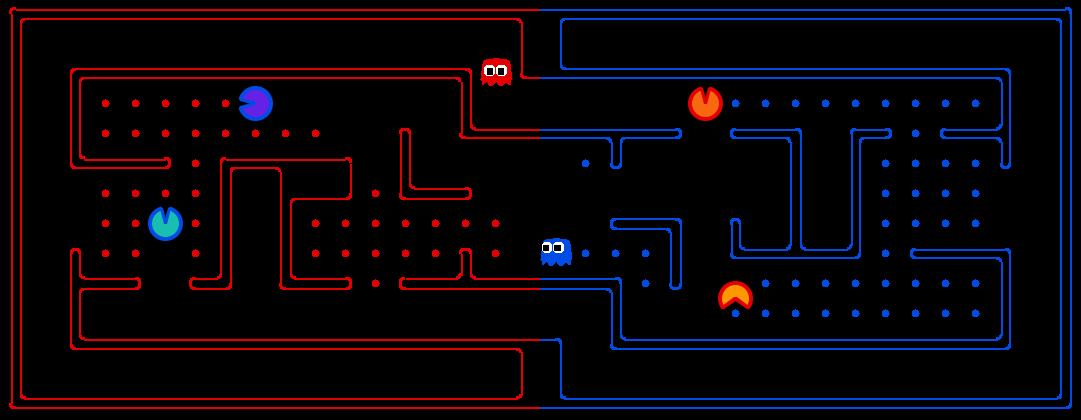
\includegraphics[width=1\linewidth]{figures/pacman}
    \caption{Pacman Capture the Flag}
  \end{figure}

\end{frame}

\begin{frame}
  \frametitle{The 2k botprize\cite{3}}
  In the contest, bots try to convince a panel of expert judges that they are actually human players.
  \begin{figure}
    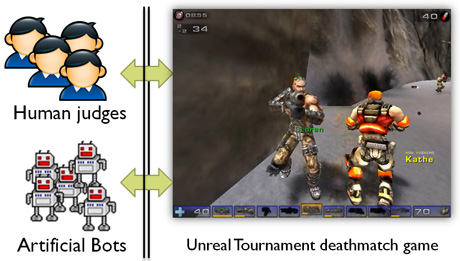
\includegraphics[width=1\linewidth]{figures/botprize}
    \caption{BotPrize judging protocol}
  \end{figure}

\end{frame}

\begin{frame}
  \frametitle{The physical travelling salesman problem competition\cite{4}}
  It is a classic algorithmic problem in the field of computer science and operations research. It is focused on optimization.
  \begin{figure}
    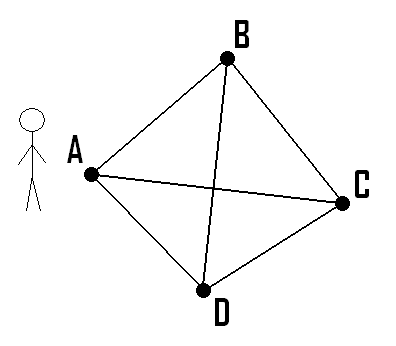
\includegraphics[width=0.6\linewidth]{figures/Salesman}
    \caption{A salesman wants to visit all cities,A, B, C and D. What is the best way to do this}
  \end{figure}
\end{frame}
%------------------------------------------------

\section{Application}

\begin{frame}
  \frametitle{Applications}

  

\end{frame}
\subsection{AlphaGo}
\begin{frame}
  \frametitle{AlphaGo - Neural Network and Tree Search}
  Sliver et.al. \cite{5} introduce a new approach to computer Go that uses ‘value networks’ to evaluate board positions and ‘policy networks’ to select moves.
  \begin{figure}
    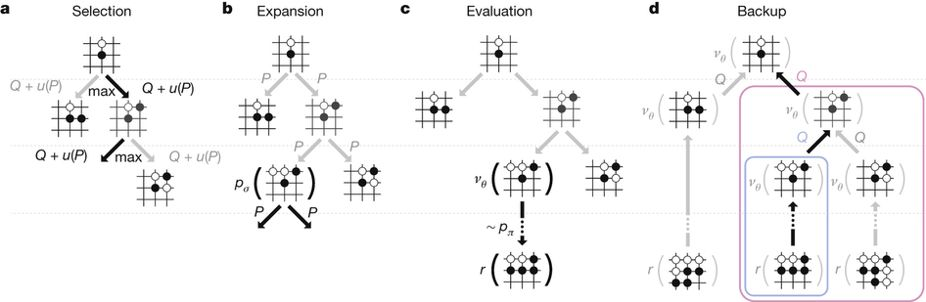
\includegraphics[width=1\linewidth]{figures/gosearch}
    \caption{ Monte Carlo tree search in AlphaGo}
  \end{figure}
\end{frame}

\subsection{StarCraft}
\begin{frame}
  \frametitle{Reinforcement Learning Applied to StarCraft}
  Wender and Watson did some research \cite{6} on applying reinforcement learning (RL) to tiny scale combat in StarCraft, aiming to design an agent performing unsupervised learning in complex environment. The result showed the viability of RL algorithms in SC.
  \begin{figure}
    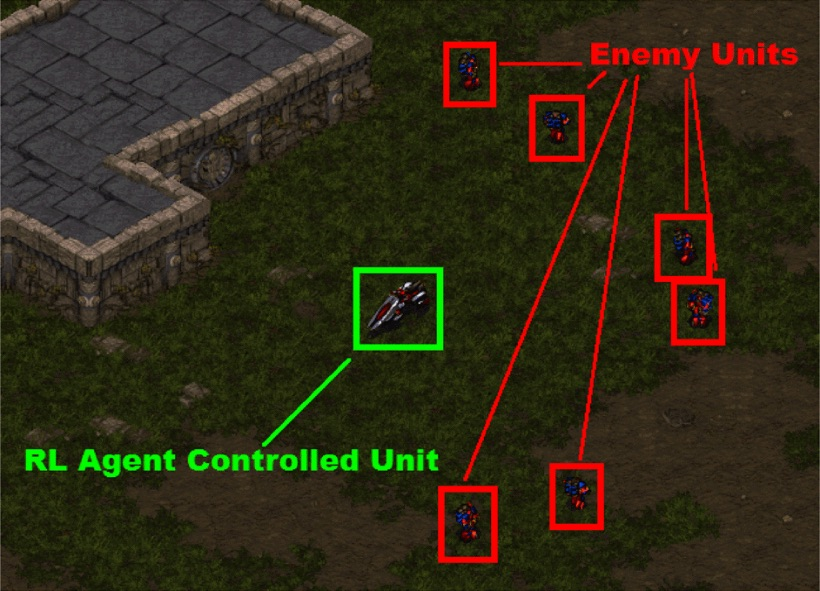
\includegraphics[width=0.6\linewidth]{figures/sc}
    \caption{ Initial unit positioning for the experimental evaluation}
  \end{figure}
\end{frame}

\subsection{Atari Games}
\begin{frame}
  \frametitle{Deep Reinforcement Learning Applied to Atari Games}
  Mnih et.al \cite{7} applied convolutional neural network trained with a variant of Q-learning to seven Atari 2600 games from the Arcade Learning Environment. The AI reached the expert level of human-like player.
  \begin{figure}
    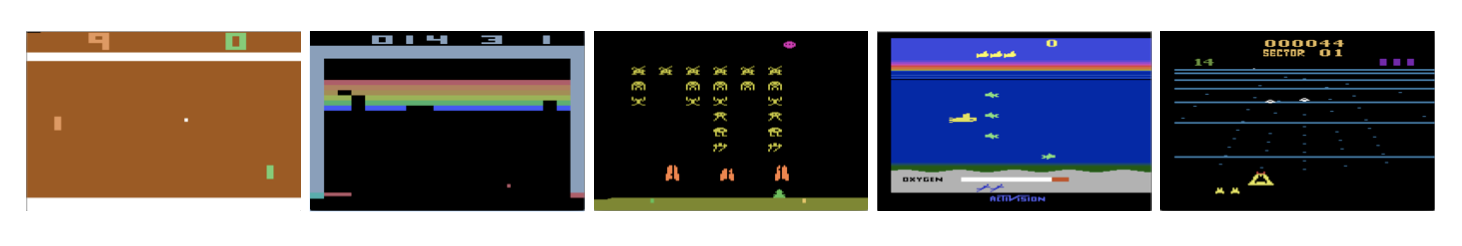
\includegraphics[width=1\linewidth]{figures/atari}
    \caption{  Screen shots from five Atari 2600 Games: (Left-to-right) Pong, Breakout, Space Invaders, Seaquest, Beam Rider}
  \end{figure}
\end{frame}


\begin{frame}[allowframebreaks]
\frametitle{References}
\footnotesize{
\begin{thebibliography}{99} % Beamer does not support BibTeX so references must be inserted manually as below
    \bibitem{1}
    R{\'e}mi Coulom.
    \newblock Efficient selectivity and backup operators in monte-carlo tree search.
    \newblock In {\em International conference on computers and games}, pages 72--83. Springer, 2006.

    \bibitem{2}
    Simon M. Lucas. 
    \newblock Ms pac-man competition. 
    \newblock In http://cswww.essex.ac.uk/staff/sml/pacman/PacManContest.html, 2012.

    \bibitem{3}
    Philip Hingston.
    \newblock The 2k botprize.
    \newblock http://botprize.org/, 2012.

    \bibitem{4}
    Diego Perez, David Robles, and Philipp Rohlfshagen. 
    \newblock The physical travelling salesman problem competition. 
    \newblock In http://www.ptsp-game.net/, 2012. 
    
    \bibitem{5}
    David Silver, Aja Huang, Chris~J Maddison, Arthur Guez, Laurent Sifre, George Van Den~Driessche, Julian Schrittwieser, Ioannis Antonoglou, Veda Panneershelvam, Marc Lanctot, et~al.
    \newblock Mastering the game of go with deep neural networks and tree search.
    \newblock In {\em nature}, 529(7587):484, 2016.

    \bibitem{6}
    S.~{Wender} and I.~{Watson}.
    \newblock Applying reinforcement learning to small scale combat in the real-time strategy game starcraft:broodwar.
    \newblock In {\em 2012 IEEE Conference on Computational Intelligence and Games (CIG)}, pages 402--408, Sep. 2012.

    \bibitem{7}
    Volodymyr Mnih, Koray Kavukcuoglu, David Silver, Alex Graves, Ioannis Antonoglou, Daan Wierstra, and Martin Riedmiller.
    \newblock Playing atari with deep reinforcement learning, 2013.
    \end{thebibliography}
}
\end{frame}

%------------------------------------------------

\begin{frame}
\Huge{\centerline{The End}}
\end{frame}

%----------------------------------------------------------------------------------------

\end{document} 